\documentclass[a4paper,10pt]{article}
\usepackage{tikz}
\usepackage{times}
% \usepackage{picins}
\usepackage{color}
\usepackage{algorithmic}
\usepackage{algorithm}
\usepackage{graphicx}
\usepackage{subfig}
\usepackage{theorem}
\usepackage{pgf}
\usepackage{tikz}
\usetikzlibrary{arrows,automata,shapes,shadows,calc}
\usepackage{amsmath,amssymb}
\usepackage[]{todo}

\usepackage{xspace}
\usepackage{tabularx}
\usepackage{colortbl}
\usepackage{nicefrac}
\usepackage{stackengine}
\usetikzlibrary{automata,positioning}
\tikzset{initial text={},
	every state/.style={circle,minimum size=.4cm,draw=black!60,very thick,fill=black!10},
	secret/.style={minimum size=.6cm,draw=red!50,very thick,fill=red!20,rectangle},
	%     secret/.style={minimum size=.4cm,draw=red!50,very thick,fill=red!20,rectangle},
	node distance= 5cm,on grid,auto}
\newcommand\obullet[1]{\ensurestackMath{\stackon[1pt]{#1}{\mkern2mu\bullet}}}
\pagestyle{empty}
\begin{document}
	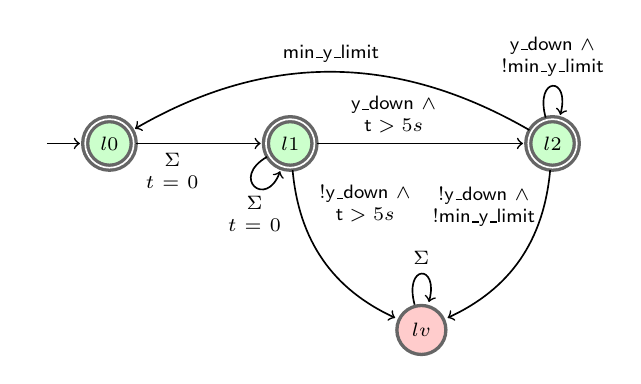
\begin{tikzpicture}[->,shorten >=1pt,auto,node distance=3.35cm,
		semithick,initial where=left, on grid]
		
		\tikzstyle{every node}=[font=\scriptsize]
		\tikzstyle{good state}=[rectangle,thick,draw=blue!75,fill=blue!20,minimum size=5mm]
		\tikzstyle{good state2}=[rectangle,thick,dashed,draw=blue!75,fill=blue!20,minimum size=5mm]
		\tikzstyle{bad state}=[circle,thick,draw=red!75,fill=red!20,minimum size=3mm]
		
		\node[ state, fill=red!20]         (lv) {$lv$};
		\node[state, accepting, fill=green!20][above left of = lv, xshift=2em](l1) {$l1$};
		\node[initial, state, accepting, fill=green!20][left of = l1, xshift=3em] (l0) {$l0$};

		\node[state, accepting, fill=green!20][above right of = lv, xshift=-2em](l2) {$l2$};
		%\node[state]       at (2.16,-0.8)  (S3)  {$l_2$};
		%\node[state, accepting]        (S4) [right of=S2, xshift= -1em] {$l_3$};
		%\node[state, accepting]        (S5) [right of=S4] {$\bullet$};
		
		
		\path
		
		(l1) edge [out=210, in=250, looseness=6]     node[below, text width=1cm, align=center] {$\Sigma$\\$t=0$} (l1)
		
		(l0) edge [yshift=-1.5em]     node[below, xshift=-1em, text width=1cm, align=center] {$\Sigma$\\$t = 0$} (l1)
		
		(l2) edge [bend right]     node[above, align=center] {$\mathsf{min\_y\_limit}$} (l0)
		
		(l1) edge  []    node[align=center, xshift=-1em] {$\mathsf{y\_down}$ $\wedge$\\ $\mathsf{t} > 5s$} (l2)
		
		%(l0) edge [loop above] node[text width=3cm, align=center] {$\lbrace \rbrace$} (l0)
		
		(l2) edge [loop above] node[align=center] {$\mathsf{y\_down}$ $\wedge$\\ $!\mathsf{min\_y\_limit}$} (l2)
		(l2) edge [bend left] node[align=center, xshift=-3.5em, yshift=3em] {$!\mathsf{y\_down}$ $\wedge$ \\ $!\mathsf{min\_y\_limit}$} (lv)
		(l1) edge [bend right] node[yshift=1em, xshift=-0.5em, align=center] {$!\mathsf{y\_down}$ $\wedge$ \\ $\mathsf{t} > 5s$} (lv)
		(lv) edge [loop above] node { $\Sigma$ } (lv) ;
		
	\end{tikzpicture}
\end{document}
